\chapter[Simulado 3]{Simulado}
\markboth{Simulado 3}{}

\vspace*{-1cm}

\num{1} Leia o título de uma notícia.

\begin{myquote}
\textbf{Governo libera mais de R\$ 1,4 milhão para socorrer o Acre}

\fonte{Agência Brasil. Governo libera mais de R\$ 1,4 milhão para socorrer o Acre.
Disponível em: \emph{https://agenciabrasil.ebc.com.br/geral/noticia/2023-03/governo-libera-mais-de-r-14-milhao-para-socorrer-o-acre}.
Acesso em: 28 mar. 2023.}
\end{myquote}

Apenas com base no título, é possível inferir que

\begin{escolha}
\item o dinheiro oferecido pelo governo ao estado do Acre não era suficiente para resolver o problema.

\item o problema do estado do Acre não se resolvia com dinheiro, apesar da liberação do governo.

\item o estado do Acre estava passando por dificuldade por ocasião da publicação da notícia.

\item o valor expresso em números é o exato que foi liberado pelo governo para o estado do Acre.
\end{escolha}



\num{2} Leia o texto a seguir e responda à pergunta:

\begin{myquote}
\textbf{Cosmonautas presos na Estação Espacial Internacional voltam em
setembro}

Tripulação russa deve encerrar uma missão espacial em março, mas não
pode deixar o espaço devido a um acidente na espaçonave MS-22.

{[}...{]}

O acidente envolveu o sistema de resfriamento da cápsula Soyuz MS-22,
que começou a vazar há dois meses. {[}...{]} Por esse motivo a equipe
não consegue deixar a Estação Espacial Internacional \textbf{(ISS, na
sigla em inglês)}. A previsão de retorno ficou para setembro deste ano,
e envolverá a substituição da parte danificada.

{[}...{]}.

\fonte{Marília Monitchele. Veja. Disponível em:
\emph{https://veja.abril.com.br/ciencia/cosmonautas-presos-na-estacao-espacial-internacional-voltam-em-setembro/}.
Acesso em: 26 fev. 2023.}
\end{myquote}

\pagebreak
O trecho destacado entre parênteses cumpre a função de

\begin{escolha}
\item apresentar uma informação acessória.

\item explicar o termo a que se relaciona.

\item traduzir a expressão relacionada.

\item enfatizar uma informação já dada.
\end{escolha}


\num{3} Leia o texto.

\begin{myquote}
{[}...{]} Na conversa de \textbf{anteontem} com Rita esqueceu-me dizer
a parte relativa a minha mulher, que lá está enterrada em Viena. Pela
segunda vez falou-me em transportá-la para o nosso jazigo. Novamente lhe
disse que estimaria muito estar perto dela, mas que, em minha opinião,
os mortos ficam bem onde caem; redarguiu-me que estão muito melhor com
os seus.

{[}...{]}.

\fonte{Joaquim Maria Machado de Assis. \emph{Memorial de Aires}.
Disponível em:
https://machado.mec.gov.br/obra-completa-lista/item/download/10\_3b418d3289f560235fccf338378de5bf.
Acesso em: 26 fev. 2023.}
\end{myquote}

\begin{tabular}{lll}
\textbf{Glossário} & \mbox{}\\
Jazigo & lugar onde se enterra.\\
Estimar & apreciar.\\
Redarguir & responder.\\
\end{tabular}\bigskip

O advérbio destacado no trecho indica

\begin{escolha}
\item o local em que um determinado fato ocorreu.

\item a negação de um determinado fato.

\item o modo como um determinado fato ocorreu.

\item o momento em que um determinado fato ocorreu.
\end{escolha}


\num{4} Leia a estrofe de um poema.
\enlargethispage{2\baselineskip}

\begin{verse}
\textbf{Orações}

As doces falas de tua alma santa\\
Valem mais do que eu valho, oh querubim!\\
Quando rezares por teu mano, à noite,\\
Não te esqueças também – reza por mim!”

\fonte{Casimiro de Abreu. Orações. In: \emph{Cantos de tristeza e
saudade.} Paris: Casa Editorial Franco-Ibero-Americana, [s.d.].}
\end{verse}

O que são as doces falas da alma?

\begin{escolha}
\item Poemas de amor.

\item Lamentações.

\item Comemorações.

\item Orações.
\end{escolha}


\num{5} Leia o texto.

\begin{myquote}
\textbf{Algoritmo: a ferramenta que faz o internauta se sentir perseguido}

Quem usa as redes sociais já deve ter se sentido perseguido por um assunto, uma propaganda ou até por sugestões de filmes para assistir. O responsável tem nome: algoritmo. É ele quem diz ao mundo digital o que nos dizer. Trata-se de uma ferramenta matemática que percebe e reorganiza os conteúdos semelhantes aos acessados pelas pessoas.

De acordo com a pesquisadora do Centro de Estudos da Sociedade da Universidade e Ciência da Universidade Federal de São Paulo (Unesp) Jade Percassi, o algoritmo registra as informações dos internautas.

{[}...{]}

Segundo Percassi, a ferramenta organiza o comportamento e entrega o conteúdo mais preciso e do interesse do usuário, como dicas de filmes e produtos. No entanto, os dados gerados nem sempre são individualizados e podem criar uma massa de informações chamada de Big Data.

{[}...{]}

\fonte{Ana Lúcia Caldas. Agência Brasil. Disponível em: \emph{https://agenciabrasil.ebc.com.br/geral/noticia/2023-03/algoritmo-ferramenta-que-faz-o-internauta-se-sentir-perseguido}. Acesso em: 29 mar. 2023.}
\end{myquote}

O operador “No entanto” cria uma

\begin{escolha}
\item consequência.

\item conclusão.

\item oposição.

\item adição.
\end{escolha}

\pagebreak
\num{6} Analise o cartaz.

\begin{figure}[htpb!]
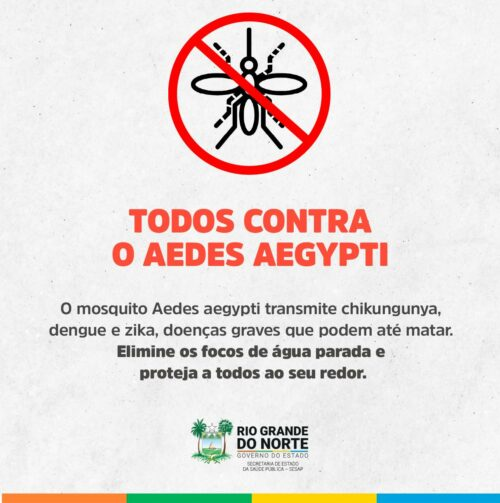
\includegraphics[width=\textwidth]{./imgs/img25.jpg}
%\caption{Fonte: https://portalcovid19.saude.rn.gov.br/noticias/sesap-orienta-populacao-para-prevencao-a-dengue-chikungunya-e-zika/. Acesso em: 26 fev. 2023.}
\end{figure}

A imagem que aparece no cartaz cumpre a função de

\begin{escolha}
\item negar o que foi escrito.

\item fortalecer o argumento pelo combate ao mosquito.

\item substituir o que foi escrito.

\item estimular a criação de focos do mosquito.
\end{escolha}


\pagebreak
\num{7} Leia o texto a seguir e responda à pergunta:

\begin{myquote}
\textbf{Manter caderneta de vacinação em dia é fundamental para prevenir
doenças}

{[}...{]}

Para além das vacinas contra a Covid-19 e Influenza, diversas outras que
compõem o calendário nacional de vacinação estão disponíveis nas salas
de vacina, localizadas nas unidades básicas de saúde (UBS). É importante
que a população se atente para a necessidade de manter em dia o esquema
de vacinação como forma de prevenir doenças para as quais já existe
imunização.

Segundo a enfermeira da área técnica de imunização da Secretaria de
Saúde, Fernanda Ledes, todas as vacinas preconizadas pelo Programa
Nacional de Imunizações (PNI), do Ministério da Saúde, e que fazem parte
do calendário nacional são extremamente importantes e devem ser
realizadas nas faixas etárias {[}...{]}. “A vacina é uma medida
preventiva, e não curativa. Devemos nos vacinar justamente para que as
doenças não circulem entre nós”, alerta. {[}...{]}.

\fonte{Geovana Albuquerque. Secretaria de Saúde do Distrito Federal. Disponível em:
\emph{https://shorturl.at/hipX8}.
Acesso em: 26 fev. 2023.}
\end{myquote}

Identifique e marque o argumento mais forte utilizado no texto para defender a
vacinação.

\begin{escolha}
\item É preciso vacinar-se para os programas de imunização serem expandidos.

\item A vacinação impede que as doenças circulem.

\item O processo de fabricação dos imunizantes será conhecido pela população.

\item É importante a vacinação apenas no calendário de imunização.
\end{escolha}


\enlargethispage{3\baselineskip}

\num{8}  Leia o texto.

\begin{myquote}
\textbf{Huka huka}\\
Com enfeites de linha, plumas e miçangas e o corpo pintado de jenipapo e
urucum, os guerreiros são convocados para o embate. Frente a frente, e
abaixados para protegerem as pernas, os oponentes
giram em forma circular e se enfrentam primeiro pelo olhar.
Posteriormente, agarram-se para ver quem consegue levantar o adversário
e levá-lo ao chão, encostando as costas no solo ou, ainda, tocar-lhe a
parte inferior do joelho, casos em que se finaliza a luta.
\end{myquote}
\pagebreak

\begin{figure}[htpb!]
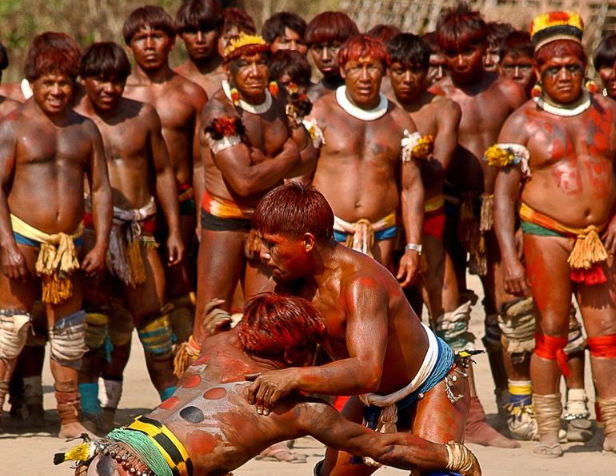
\includegraphics[width=\textwidth]{./imgs/art36.png}
\end{figure}\enlargethispage{2\baselineskip}

\fonte{Fonte de pesquisa: Fundação Nacional dos Povos Indígenas. Huka Huka, a luta corporal do Xingu, contribui para manter viva a cultura indígena no Mato Grosso. Disponível em:
\emph{https://www.gov.br/funai/pt-br/assuntos/noticias/2022-02/huka-huka-a-luta-corporal-do-xingu-contribui-para-manter-viva-a-cultura-indigena-no-mato-grosso}.
Acesso em: 26 mar. 2023.}

\noindent{}Assinale a alternativa que corresponde às características da
manifestação cultural huka huka.\looseness=-1

\begin{escolha} 
\item
  Patrimônio cultural imaterial de matriz indígena.
\item
  Patrimônio cultural material de matriz indígena.
\item
  Patrimônio cultural material transmitido de geração a geração.
\item
  Patrimônio cultural imaterial dos povos indígenas do nordeste
  brasileiro.
\end{escolha}



\num{9}  Assinale a alternativa que corresponde às linguagens artísticas presentes
no forró.

\begin{escolha}
\item
  Artes visuais e dança.
\item
  Artes visuais e música.
\item
  Dança e música.
\item
  Música e teatro.
\end{escolha}

\pagebreak
\num{10}  Leia o texto.

\begin{myquote}
Instrumento do tipo idiofone (cujo som é provocado por sua própria vibração) de agitamento feito de cabaça com sementes ou grãos secos, o que funciona como um chocalho. Serve para puxar a dança, e o pajé o utiliza para trazer bons espíritos e afugentar os maus.
\end{myquote}

O maracá, descrito no texto, é de origem

\begin{escolha}
\item
  europeia.
\item
  indígena.
\item
  africana.
\item
  desconhecida.
\end{escolha}


%\chapter*{} %Simulado 3
%\begin{figure}[htpb!]
%\vspace*{-3cm}
%\hspace*{-2.5cm}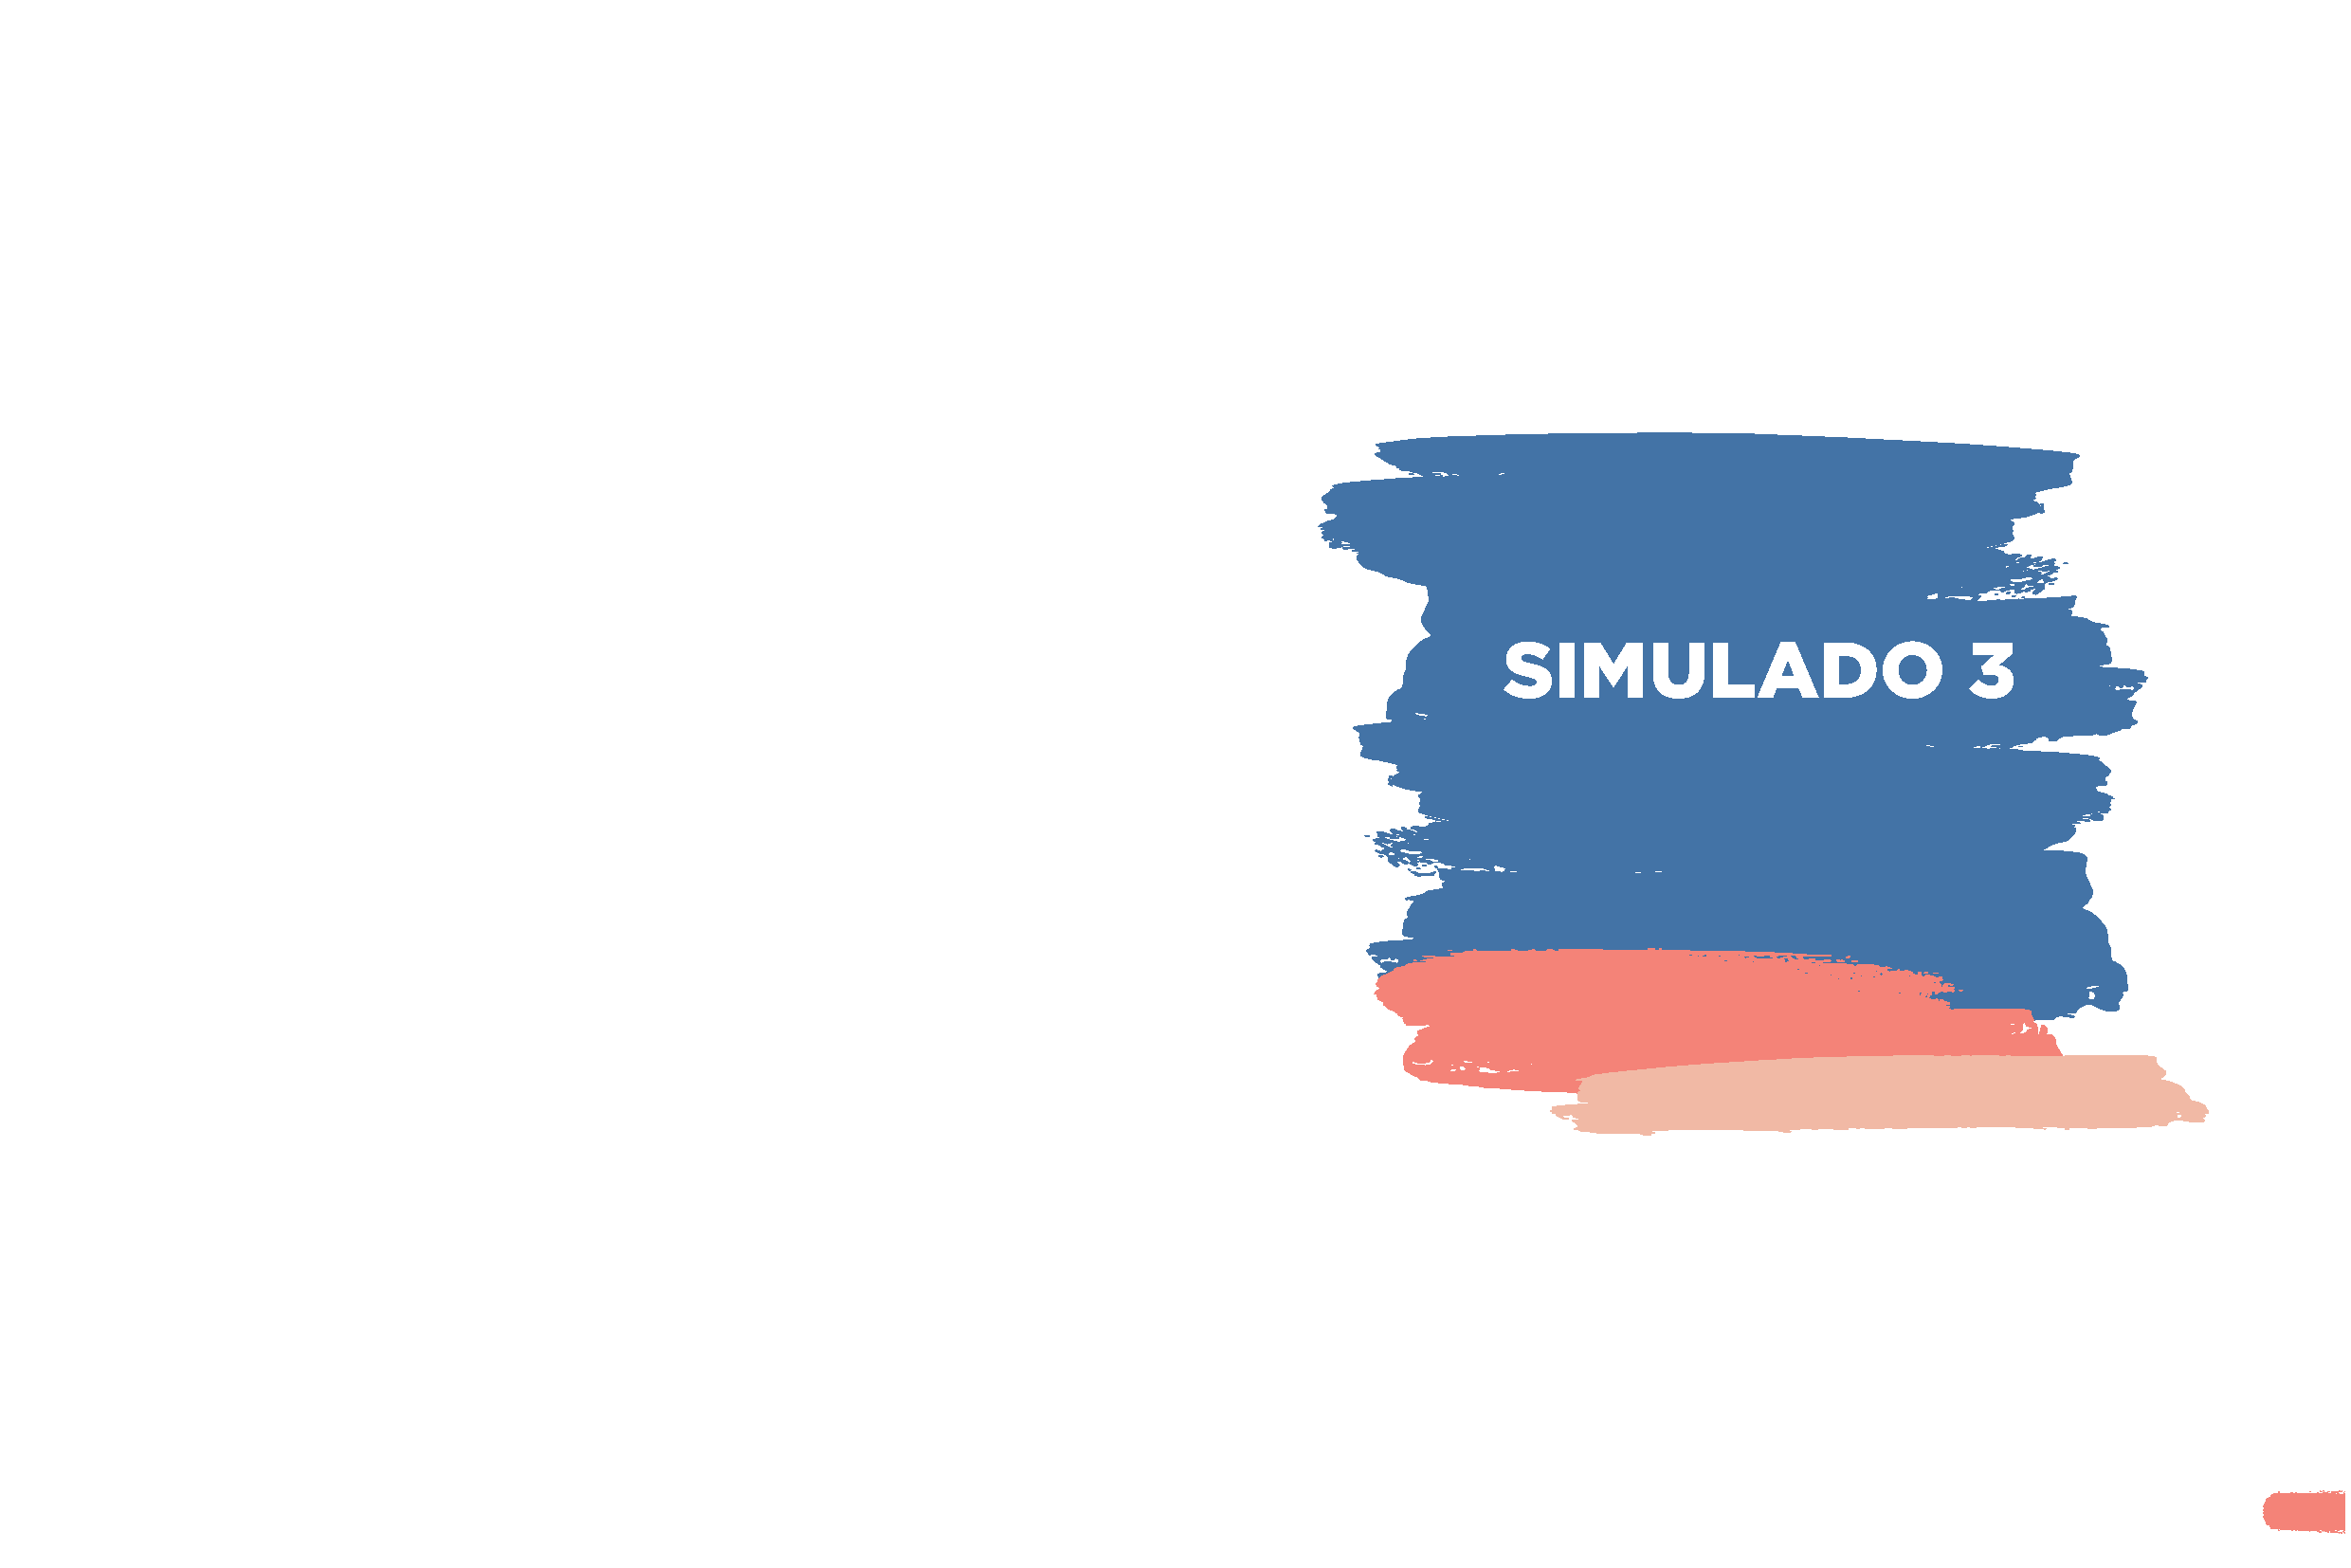
\includegraphics[scale=1]{../watermarks/3simulado5ano.pdf}
%\end{figure}
%\newwatermark[pagex={65,67}]{\vspace{2.5cm}\hspace*{8cm}\includegraphics[scale=1]{../watermarks/%bgsim5anoimpar.pdf}}
%\newwatermark[pagex={66}]{\vspace{2.5cm}\hspace*{7.8cm}\includegraphics[scale=1]{../watermarks/%bgsim5anopar.pdf}}
%
%\pagebreak
%\movetooddpage
%\markboth{Simulado 3}{}

\num{11}

\begin{myquote}
Os objetos biográficos dão significado à casa da família de Hugo e
estão guardados em seu interior, sendo que a presença deles neste lugar
dá a sensação de continuidade da vida do próprio Hugo. Embora esteja
praticamente abandonada, um dia foi habitada e nela os objetos ainda
existentes reportam a pertença a alguém que os usou no cotidiano. Como
cita Malvina Muszkat, “o sentimento de continuidade se relaciona à
dimensão tempo, no sentido de se manter único através de diferentes
tempos e de ser `conscientizado' através do exercício da memória”.

\fonte{GOMES, COSTA. A Casa e os objetos de memória. \textbf{Revista Iniciação
Científica}, Criciúma, v. 14, n. 1, 2016}
\end{myquote}

Segundo o texto, os objetos da casa de Hugo podem ser considerados

\begin{escolha}
\item ameaças ao meio ambiente.

\item lixos a serem reciclados.

\item documentos históricos.

\item bens materiais que custam muito dinheiro.
\end{escolha}


\pagebreak
\num{12} A imagem abaixo representa uma ação individual prejudicial ao meio ambiente:

\begin{figure}[htpb!]

\includegraphics[width=\textwidth]{./imgs/img68.png}
%\caption{Disponível em: \emph{https://br.freepik.com/vetores-gratis/fundo-do-corredor-da-escola-suja\_4228059.htm\#query=escola\%20lixo\&position=0\&from\_view=search\&track=ais} Acesso em: 23 fev. 2023.}
\end{figure}

\begin{escolha}
\item cortar árvores em florestas.

\item realizar reciclagem de papéis.

\item queimar plantações nos campos.

\item jogar lixo em locais inadequados.
\end{escolha}

\num{13}

\begin{myquote}
Atribui-se aos gregos, na Antiguidade, a invenção das vogais, a
difusão e adoção do alfabeto da sociedade fenícia, como também a
invenção do método de alfabetização sobre o qual podemos afirmar que
milhões de pessoas aprenderam a ler e a escrever, através dos três
milhares de anos que se passaram desde que as primeiras crianças
“cantaram” o bê-a-bá. Este método, onde se aprendia separadamente a
ler e a escrever, foi sendo adotado por outros povos, passando por
adaptações e transformações, mas, em geral, chamado simplesmente de
alfabetização.

\fonte{STAMATTO, Maria. Alfabetização Histórica em materiais didáticos:
significados e usos \textbf{ANPUH} – XXV SIMPÓSIO NACIONAL DE HISTÓRIA
– Fortaleza, 2009.}
\end{myquote}

Segundo o texto, uma importante invenção dos fenícios para nossa sociedade foi

\begin{escolha}
\item a escrita.

\item a escola.

\item o alfabeto.

\item o livro.
\end{escolha}



\num{14}

\begin{myquote}
Em geral, a base da organização social de um povo indígena é a
família extensa, entendida como uma unidade social articulada em torno
de um patriarca ou de uma matriarca por meio de relações de parentesco
ou afinidade política ou econômica. São denominadas famílias extensas
por aglutinarem um número de pessoas e de famílias muito maior que uma
família tradicional europeia. Uma família extensa indígena geralmente
reúne a família do patriarca ou da matriarca, as famílias dos filhos,
dos genros, das noras, dos cunhados e outras famílias afins que se
filiam à grande família por interesses específicos.

\fonte{DOS SANTOS, Luciano(Baniwa). \textbf{O índio brasileiro.} Secretaria de
Educação Continuada, Alfabetização e Diversidade (Secad), Organização
das Nações Unidas para a Educação, a Ciência e a Cultura (Unesco) e
Projeto Trilhas de Conhecimentos – LACED/Museu Nacional, 2006.}
\end{myquote}

\noindent{}Segundo o texto, a família extensa é, para os indígenas,

\begin{escolha}
\item uma organização proibida nas aldeias.

\item uma lenda contada pelos mais velhos.

\item uma junção de vários grupos familiares.

\item um outro nome para se chamar o povo nativo.
\end{escolha}


\pagebreak
\num{15}

\begin{myquote}
\textbf{Campanha pela Valorização do Trabalho Doméstico}

Queremos trazer para pauta das discussões da sociedade a questão do
trabalho doméstico remunerado com o objetivo de sensibilizar a sociedade
civil e os agentes públicos para o reconhecimento dos direitos das
trabalhadoras domésticas, pela igualdade de direitos com as demais
categorias. {[}\ldots{}{]}
São consideradas trabalhadoras domésticas as pessoas maiores
de 18 anos que prestam serviço de natureza contínua (com frequência) e
de finalidade não lucrativa à pessoa ou à família, no espaço residencial
destas. {[}\ldots{}{]}

\fonte{Centro de ação cultural. Campanha pela valorização do trabalho doméstico. Disponível em:
\emph{https://centrac.org.br/publicacoes/campanhas/campanha-pela-valorizacao-do-trabalho-domestico/}.
Acesso em: 23 fev. 2023.}
\end{myquote}

\noindent{}Um exemplo de trabalhadora doméstica e sua importância é

\begin{escolha}
\item a secretária, que organiza as coisas dentro de um escritório.

\item a padeira, que produz os pães a serem vendidos na padaria.

\item a vendedora, que mostra os produtos disponíveis na loja.

\item a faxineira, que mantém a limpeza do ambiente da casa.
\end{escolha}




\pagebreak